\documentclass[12pt]{article}
\usepackage[table]{xcolor}
\usepackage[shortlabels]{enumitem}
\usepackage{tabularx,xltabular}
\usepackage{graphicx}
\usepackage{hyperref}
\usepackage{verbatim}
\usepackage{geometry}
\usepackage{ulem}
\usepackage[official]{eurosym}
\usepackage{tikz}
\usetikzlibrary{arrows,backgrounds,calc,decorations.markings,patterns,3d}
\usepackage{pgfplots}
\pgfplotsset{compat = newest}
\usetikzlibrary{fit}
\newcommand\addvmargin[1]{
\usetikzlibrary{arrows}
\node[fit=(current bounding box),inner ysep=#1,inner xsep=0]{};}
\usepackage{cancel}
\usepackage{fontspec}
\usepackage{array}  
\geometry{a4paper, top=2cm, left=2cm, right=2cm, bottom=2cm, headsep=1cm}
\usepackage{tabu}
\usepackage{pst-node}
\usepackage{colortbl}
\usepackage{array}
\usepackage{german}
\setlength\parindent{0pt}
\newcolumntype{?}{!{\vrule width 1pt}}
\usepackage{makecell}
\renewcommand{\arraystretch}{2.5}
\usepackage{pbox}
\usepackage{amssymb}
\usepackage{amsmath}
\usepackage{booktabs}
\newcolumntype{L}[1]{>{\raggedright\let\newline\\\arraybackslash\hspace{0pt}}m{#1}}
\newcolumntype{C}[1]{>{\centering\let\newline\\\arraybackslash\hspace{0pt}}m{#1}}
\newcolumntype{R}[1]{>{\raggedleft\let\newline\\\arraybackslash\hspace{0pt}}m{#1}}
\begin{document}
\rightline{Datum: 08.06.2023}
\centerline{{\Large Tägliche Übungen}} 
\vspace{1cm}
\noindent \\


\begin{xltabular}{\textwidth}{|C{0.75cm}|X|C{0.75cm}|X|}
\arrayrulecolor{black}\hline
a)&Berechne die Variable $$14\cdot y-10=74$$
&
b)&Berechne die Variable $$14\cdot y-16=110$$
\\\hline
c)&Berechne die Variable $$12\cdot b-9=111$$
&
d)&Berechne die Variable $$13\cdot x-7=110$$
\\\hline
e)&Berechne die Variable $$6\cdot a-16=2$$
&
f)&Berechne die Variable $$7\cdot b-9=75$$
\\\hline
g)&Berechne die Variable $$10\cdot a-20=100$$
&
h)&Berechne die Variable $$3\cdot y-19=-13$$
\\\hline
i)&Berechne die Variable $$9\cdot x-20=61$$
&
j)&Berechne die Variable $$2\cdot y-6=10$$
\\\hline
k)&Berechne die Variable $$10\cdot b-10=100$$
&
l)&Berechne die Variable $$15\cdot a-9=141$$
\\\hline
m)&Berechne die Variable $$6\cdot y-7=59$$
&
n)&Berechne die Variable $$5\cdot b-13=2$$
\\\hline
o)&Berechne die Variable $$13\cdot x-13=91$$
&
p)&Berechne die Variable $$14\cdot a-14=84$$
\\\hline
q)&Berechne die Variable $$6\cdot b-13=17$$
&
r)&Berechne die Variable $$3\cdot a-4=11$$
\\\hline
s)&Berechne die Variable $$2\cdot x-5=15$$
&
t)&Berechne die Variable $$9\cdot y-12=42$$
\\\hline
u)&Berechne die Variable $$7\cdot b-3=53$$
&
v)&Berechne die Variable $$15\cdot b-16=134$$
\\\hline
w)&Berechne die Variable $$8\cdot y-11=85$$
&
x)&Berechne die Variable $$15\cdot x-14=106$$
\\\hline
y)&Berechne die Variable $$5\cdot a-3=7$$
&
z)&Berechne die Variable $$14\cdot b-12=114$$
\\\hline
\end{xltabular}
\vspace{0.5cm}
\newpage
\rightline{Datum: 08.06.2023}
\centerline{{\large Lösungen Tägliche Übungen}} 
\vspace{0.5cm}

\begin{xltabular}{\textwidth}{|C{0.75cm}|X|C{0.75cm}|X|}
\arrayrulecolor{black}\hline
a)&\begingroup\setlength{\jot}{-0.03cm}
\tikzstyle{background grid}=[draw, black!15,step=.5cm]
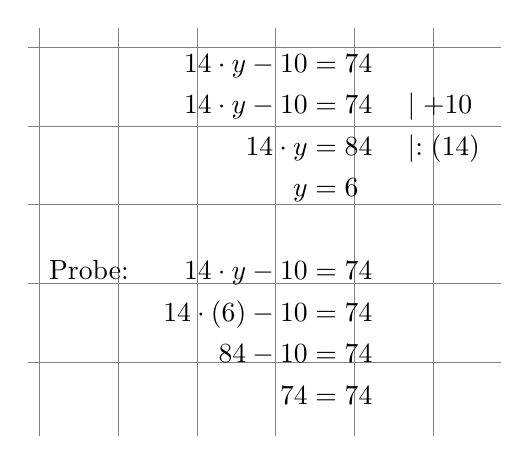
\begin{tikzpicture}[show background grid]
\node[below right] at (0,0.1) {
$\begin{aligned}
14\cdot y-10 &=74& &  \\
14\cdot y - 10 &=74& & \mid + 10\\
14\cdot y &=84& & \mid :\left(14\right)\\
y &=6& & 
\\
\\
\mbox{Probe:}\qquad 14\cdot y-10 &=74& &  \\
14\cdot \left(6\right)-10 &=74& &  \\
84-10 &=74& &  \\
74 &=74& &  \\
\end{aligned}$};
\end{tikzpicture}
\endgroup
&
b)&\begingroup\setlength{\jot}{-0.03cm}
\tikzstyle{background grid}=[draw, black!15,step=.5cm]
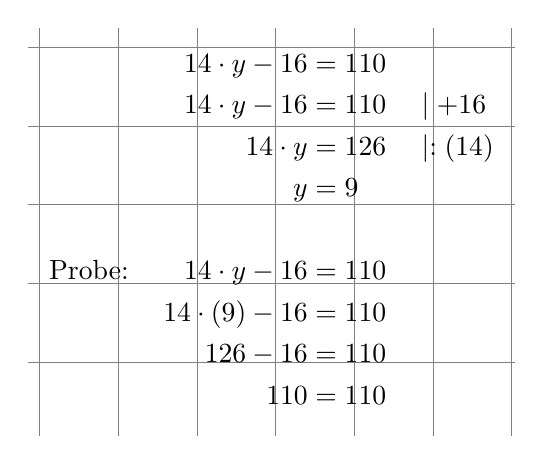
\begin{tikzpicture}[show background grid]
\node[below right] at (0,0.1) {
$\begin{aligned}
14\cdot y-16 &=110& &  \\
14\cdot y - 16 &=110& & \mid + 16\\
14\cdot y &=126& & \mid :\left(14\right)\\
y &=9& & 
\\
\\
\mbox{Probe:}\qquad 14\cdot y-16 &=110& &  \\
14\cdot \left(9\right)-16 &=110& &  \\
126-16 &=110& &  \\
110 &=110& &  \\
\end{aligned}$};
\end{tikzpicture}
\endgroup
\\\hline
c)&\begingroup\setlength{\jot}{-0.03cm}
\tikzstyle{background grid}=[draw, black!15,step=.5cm]
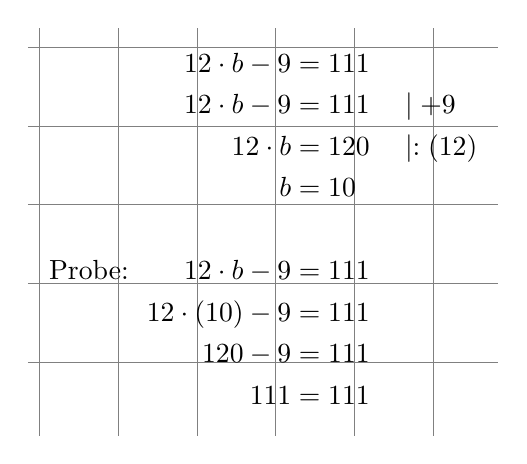
\begin{tikzpicture}[show background grid]
\node[below right] at (0,0.1) {
$\begin{aligned}
12\cdot b-9 &=111& &  \\
12\cdot b - 9 &=111& & \mid + 9\\
12\cdot b &=120& & \mid :\left(12\right)\\
b &=10& & 
\\
\\
\mbox{Probe:}\qquad 12\cdot b-9 &=111& &  \\
12\cdot \left(10\right)-9 &=111& &  \\
120-9 &=111& &  \\
111 &=111& &  \\
\end{aligned}$};
\end{tikzpicture}
\endgroup
&
d)&\begingroup\setlength{\jot}{-0.03cm}
\tikzstyle{background grid}=[draw, black!15,step=.5cm]
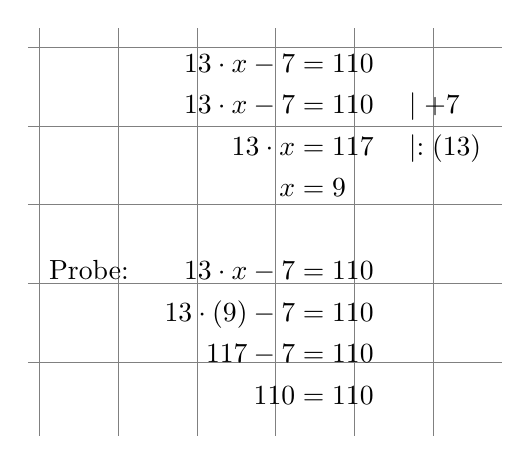
\begin{tikzpicture}[show background grid]
\node[below right] at (0,0.1) {
$\begin{aligned}
13\cdot x-7 &=110& &  \\
13\cdot x - 7 &=110& & \mid + 7\\
13\cdot x &=117& & \mid :\left(13\right)\\
x &=9& & 
\\
\\
\mbox{Probe:}\qquad 13\cdot x-7 &=110& &  \\
13\cdot \left(9\right)-7 &=110& &  \\
117-7 &=110& &  \\
110 &=110& &  \\
\end{aligned}$};
\end{tikzpicture}
\endgroup
\\\hline
e)&\begingroup\setlength{\jot}{-0.03cm}
\tikzstyle{background grid}=[draw, black!15,step=.5cm]
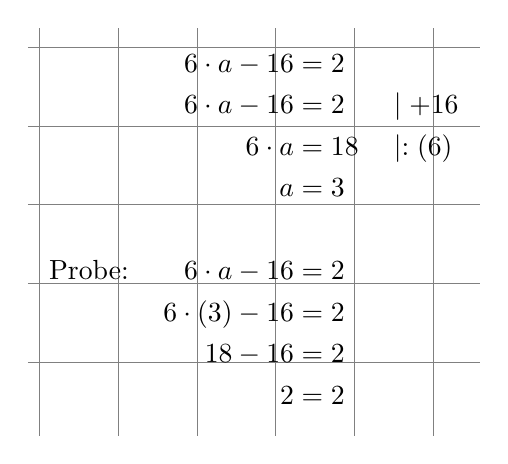
\begin{tikzpicture}[show background grid]
\node[below right] at (0,0.1) {
$\begin{aligned}
6\cdot a-16 &=2& &  \\
6\cdot a - 16 &=2& & \mid + 16\\
6\cdot a &=18& & \mid :\left(6\right)\\
a &=3& & 
\\
\\
\mbox{Probe:}\qquad 6\cdot a-16 &=2& &  \\
6\cdot \left(3\right)-16 &=2& &  \\
18-16 &=2& &  \\
2 &=2& &  \\
\end{aligned}$};
\end{tikzpicture}
\endgroup
&
f)&\begingroup\setlength{\jot}{-0.03cm}
\tikzstyle{background grid}=[draw, black!15,step=.5cm]
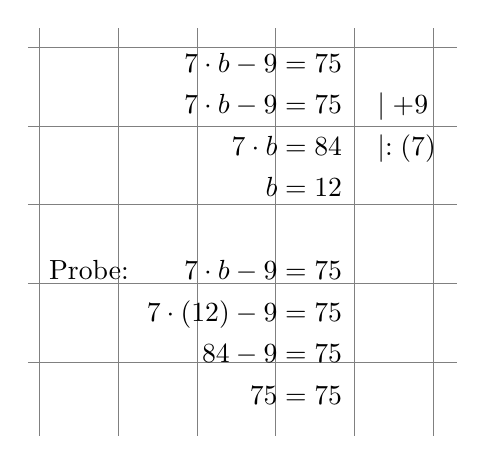
\begin{tikzpicture}[show background grid]
\node[below right] at (0,0.1) {
$\begin{aligned}
7\cdot b-9 &=75& &  \\
7\cdot b - 9 &=75& & \mid + 9\\
7\cdot b &=84& & \mid :\left(7\right)\\
b &=12& & 
\\
\\
\mbox{Probe:}\qquad 7\cdot b-9 &=75& &  \\
7\cdot \left(12\right)-9 &=75& &  \\
84-9 &=75& &  \\
75 &=75& &  \\
\end{aligned}$};
\end{tikzpicture}
\endgroup
\\\hline
g)&\begingroup\setlength{\jot}{-0.03cm}
\tikzstyle{background grid}=[draw, black!15,step=.5cm]
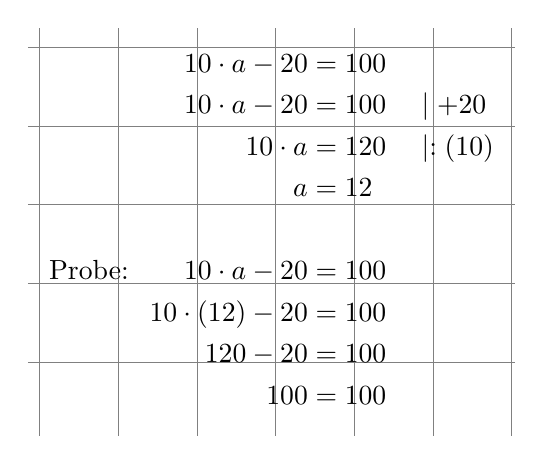
\begin{tikzpicture}[show background grid]
\node[below right] at (0,0.1) {
$\begin{aligned}
10\cdot a-20 &=100& &  \\
10\cdot a - 20 &=100& & \mid + 20\\
10\cdot a &=120& & \mid :\left(10\right)\\
a &=12& & 
\\
\\
\mbox{Probe:}\qquad 10\cdot a-20 &=100& &  \\
10\cdot \left(12\right)-20 &=100& &  \\
120-20 &=100& &  \\
100 &=100& &  \\
\end{aligned}$};
\end{tikzpicture}
\endgroup
&
h)&\begingroup\setlength{\jot}{-0.03cm}
\tikzstyle{background grid}=[draw, black!15,step=.5cm]
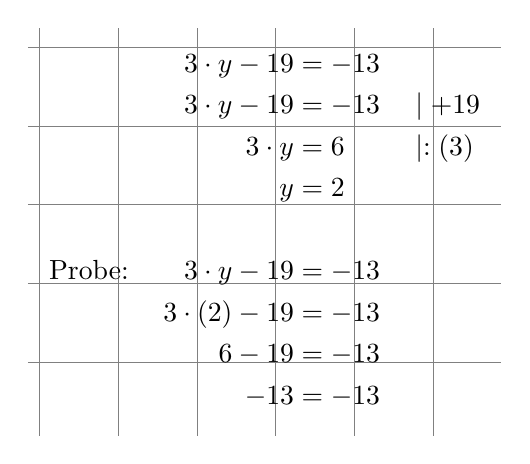
\begin{tikzpicture}[show background grid]
\node[below right] at (0,0.1) {
$\begin{aligned}
3\cdot y-19 &=-13& &  \\
3\cdot y - 19 &=-13& & \mid + 19\\
3\cdot y &=6& & \mid :\left(3\right)\\
y &=2& & 
\\
\\
\mbox{Probe:}\qquad 3\cdot y-19 &=-13& &  \\
3\cdot \left(2\right)-19 &=-13& &  \\
6-19 &=-13& &  \\
-13 &=-13& &  \\
\end{aligned}$};
\end{tikzpicture}
\endgroup
\\\hline
i)&\begingroup\setlength{\jot}{-0.03cm}
\tikzstyle{background grid}=[draw, black!15,step=.5cm]
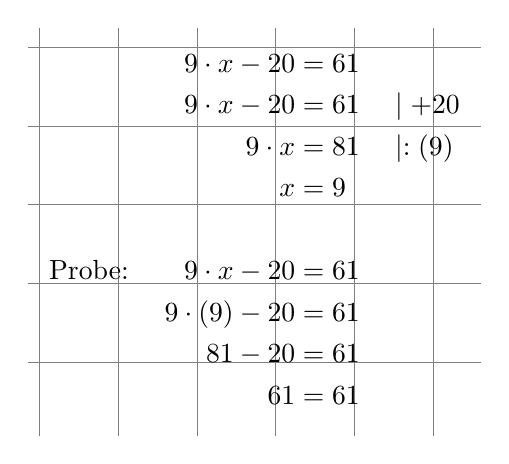
\begin{tikzpicture}[show background grid]
\node[below right] at (0,0.1) {
$\begin{aligned}
9\cdot x-20 &=61& &  \\
9\cdot x - 20 &=61& & \mid + 20\\
9\cdot x &=81& & \mid :\left(9\right)\\
x &=9& & 
\\
\\
\mbox{Probe:}\qquad 9\cdot x-20 &=61& &  \\
9\cdot \left(9\right)-20 &=61& &  \\
81-20 &=61& &  \\
61 &=61& &  \\
\end{aligned}$};
\end{tikzpicture}
\endgroup
&
j)&\begingroup\setlength{\jot}{-0.03cm}
\tikzstyle{background grid}=[draw, black!15,step=.5cm]
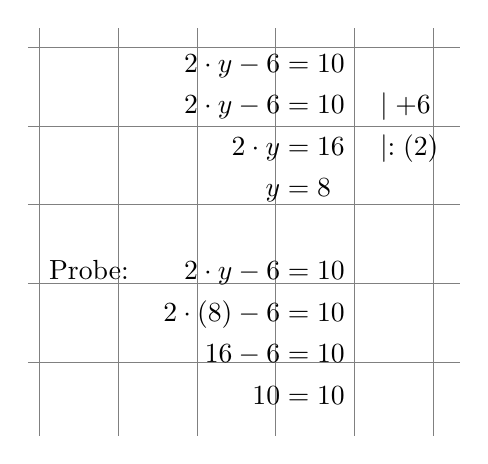
\begin{tikzpicture}[show background grid]
\node[below right] at (0,0.1) {
$\begin{aligned}
2\cdot y-6 &=10& &  \\
2\cdot y - 6 &=10& & \mid + 6\\
2\cdot y &=16& & \mid :\left(2\right)\\
y &=8& & 
\\
\\
\mbox{Probe:}\qquad 2\cdot y-6 &=10& &  \\
2\cdot \left(8\right)-6 &=10& &  \\
16-6 &=10& &  \\
10 &=10& &  \\
\end{aligned}$};
\end{tikzpicture}
\endgroup
\\\hline
k)&\begingroup\setlength{\jot}{-0.03cm}
\tikzstyle{background grid}=[draw, black!15,step=.5cm]
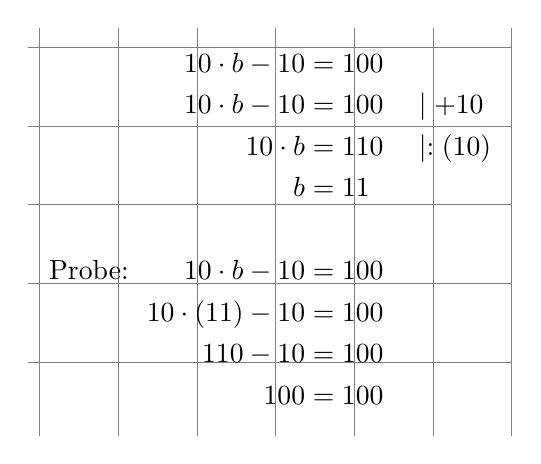
\begin{tikzpicture}[show background grid]
\node[below right] at (0,0.1) {
$\begin{aligned}
10\cdot b-10 &=100& &  \\
10\cdot b - 10 &=100& & \mid + 10\\
10\cdot b &=110& & \mid :\left(10\right)\\
b &=11& & 
\\
\\
\mbox{Probe:}\qquad 10\cdot b-10 &=100& &  \\
10\cdot \left(11\right)-10 &=100& &  \\
110-10 &=100& &  \\
100 &=100& &  \\
\end{aligned}$};
\end{tikzpicture}
\endgroup
&
l)&\begingroup\setlength{\jot}{-0.03cm}
\tikzstyle{background grid}=[draw, black!15,step=.5cm]
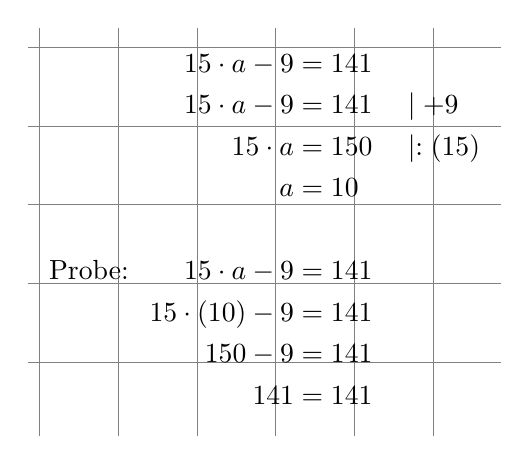
\begin{tikzpicture}[show background grid]
\node[below right] at (0,0.1) {
$\begin{aligned}
15\cdot a-9 &=141& &  \\
15\cdot a - 9 &=141& & \mid + 9\\
15\cdot a &=150& & \mid :\left(15\right)\\
a &=10& & 
\\
\\
\mbox{Probe:}\qquad 15\cdot a-9 &=141& &  \\
15\cdot \left(10\right)-9 &=141& &  \\
150-9 &=141& &  \\
141 &=141& &  \\
\end{aligned}$};
\end{tikzpicture}
\endgroup
\\\hline
m)&\begingroup\setlength{\jot}{-0.03cm}
\tikzstyle{background grid}=[draw, black!15,step=.5cm]
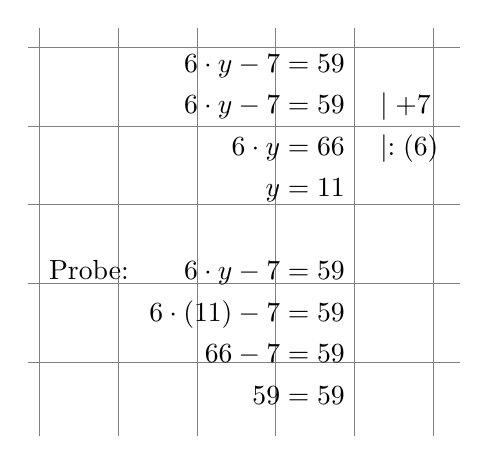
\begin{tikzpicture}[show background grid]
\node[below right] at (0,0.1) {
$\begin{aligned}
6\cdot y-7 &=59& &  \\
6\cdot y - 7 &=59& & \mid + 7\\
6\cdot y &=66& & \mid :\left(6\right)\\
y &=11& & 
\\
\\
\mbox{Probe:}\qquad 6\cdot y-7 &=59& &  \\
6\cdot \left(11\right)-7 &=59& &  \\
66-7 &=59& &  \\
59 &=59& &  \\
\end{aligned}$};
\end{tikzpicture}
\endgroup
&
n)&\begingroup\setlength{\jot}{-0.03cm}
\tikzstyle{background grid}=[draw, black!15,step=.5cm]
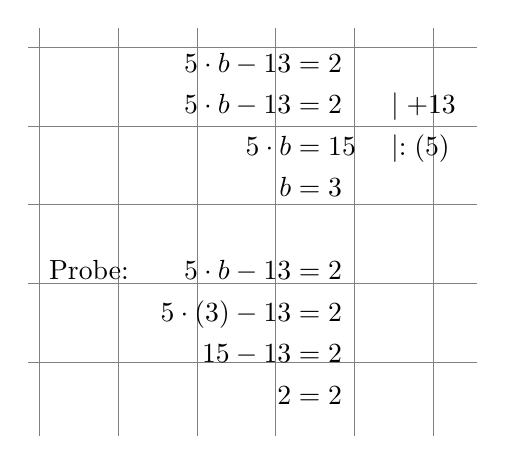
\begin{tikzpicture}[show background grid]
\node[below right] at (0,0.1) {
$\begin{aligned}
5\cdot b-13 &=2& &  \\
5\cdot b - 13 &=2& & \mid + 13\\
5\cdot b &=15& & \mid :\left(5\right)\\
b &=3& & 
\\
\\
\mbox{Probe:}\qquad 5\cdot b-13 &=2& &  \\
5\cdot \left(3\right)-13 &=2& &  \\
15-13 &=2& &  \\
2 &=2& &  \\
\end{aligned}$};
\end{tikzpicture}
\endgroup
\\\hline
o)&\begingroup\setlength{\jot}{-0.03cm}
\tikzstyle{background grid}=[draw, black!15,step=.5cm]
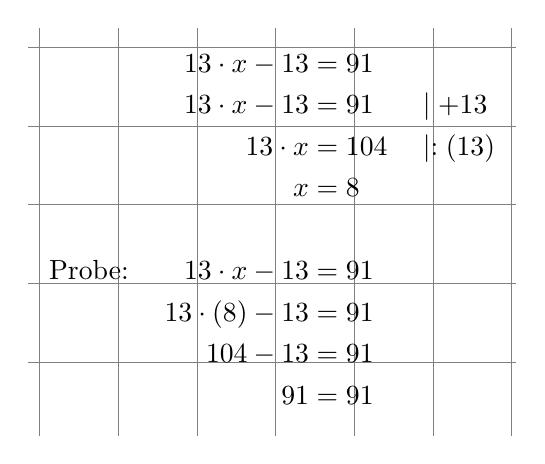
\begin{tikzpicture}[show background grid]
\node[below right] at (0,0.1) {
$\begin{aligned}
13\cdot x-13 &=91& &  \\
13\cdot x - 13 &=91& & \mid + 13\\
13\cdot x &=104& & \mid :\left(13\right)\\
x &=8& & 
\\
\\
\mbox{Probe:}\qquad 13\cdot x-13 &=91& &  \\
13\cdot \left(8\right)-13 &=91& &  \\
104-13 &=91& &  \\
91 &=91& &  \\
\end{aligned}$};
\end{tikzpicture}
\endgroup
&
p)&\begingroup\setlength{\jot}{-0.03cm}
\tikzstyle{background grid}=[draw, black!15,step=.5cm]
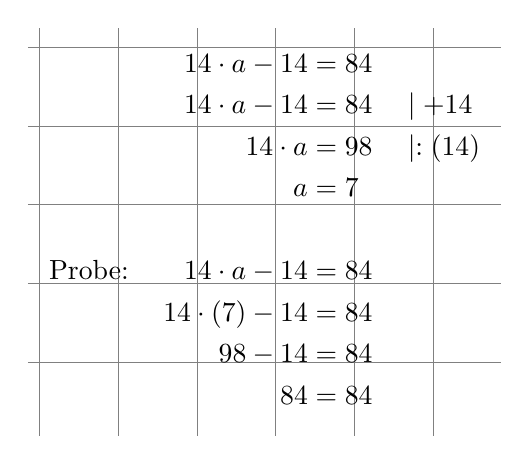
\begin{tikzpicture}[show background grid]
\node[below right] at (0,0.1) {
$\begin{aligned}
14\cdot a-14 &=84& &  \\
14\cdot a - 14 &=84& & \mid + 14\\
14\cdot a &=98& & \mid :\left(14\right)\\
a &=7& & 
\\
\\
\mbox{Probe:}\qquad 14\cdot a-14 &=84& &  \\
14\cdot \left(7\right)-14 &=84& &  \\
98-14 &=84& &  \\
84 &=84& &  \\
\end{aligned}$};
\end{tikzpicture}
\endgroup
\\\hline
q)&\begingroup\setlength{\jot}{-0.03cm}
\tikzstyle{background grid}=[draw, black!15,step=.5cm]
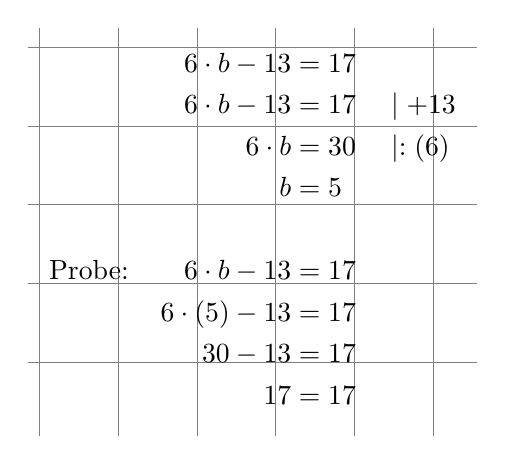
\begin{tikzpicture}[show background grid]
\node[below right] at (0,0.1) {
$\begin{aligned}
6\cdot b-13 &=17& &  \\
6\cdot b - 13 &=17& & \mid + 13\\
6\cdot b &=30& & \mid :\left(6\right)\\
b &=5& & 
\\
\\
\mbox{Probe:}\qquad 6\cdot b-13 &=17& &  \\
6\cdot \left(5\right)-13 &=17& &  \\
30-13 &=17& &  \\
17 &=17& &  \\
\end{aligned}$};
\end{tikzpicture}
\endgroup
&
r)&\begingroup\setlength{\jot}{-0.03cm}
\tikzstyle{background grid}=[draw, black!15,step=.5cm]
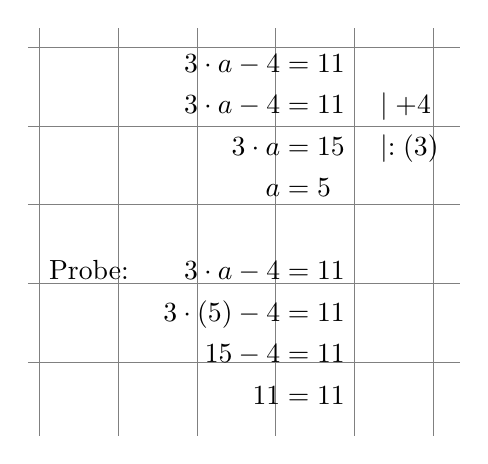
\begin{tikzpicture}[show background grid]
\node[below right] at (0,0.1) {
$\begin{aligned}
3\cdot a-4 &=11& &  \\
3\cdot a - 4 &=11& & \mid + 4\\
3\cdot a &=15& & \mid :\left(3\right)\\
a &=5& & 
\\
\\
\mbox{Probe:}\qquad 3\cdot a-4 &=11& &  \\
3\cdot \left(5\right)-4 &=11& &  \\
15-4 &=11& &  \\
11 &=11& &  \\
\end{aligned}$};
\end{tikzpicture}
\endgroup
\\\hline
s)&\begingroup\setlength{\jot}{-0.03cm}
\tikzstyle{background grid}=[draw, black!15,step=.5cm]
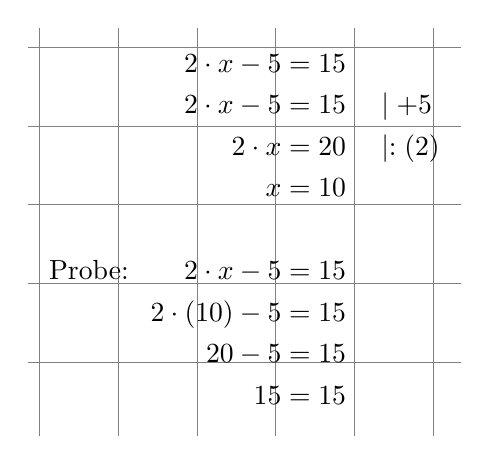
\begin{tikzpicture}[show background grid]
\node[below right] at (0,0.1) {
$\begin{aligned}
2\cdot x-5 &=15& &  \\
2\cdot x - 5 &=15& & \mid + 5\\
2\cdot x &=20& & \mid :\left(2\right)\\
x &=10& & 
\\
\\
\mbox{Probe:}\qquad 2\cdot x-5 &=15& &  \\
2\cdot \left(10\right)-5 &=15& &  \\
20-5 &=15& &  \\
15 &=15& &  \\
\end{aligned}$};
\end{tikzpicture}
\endgroup
&
t)&\begingroup\setlength{\jot}{-0.03cm}
\tikzstyle{background grid}=[draw, black!15,step=.5cm]
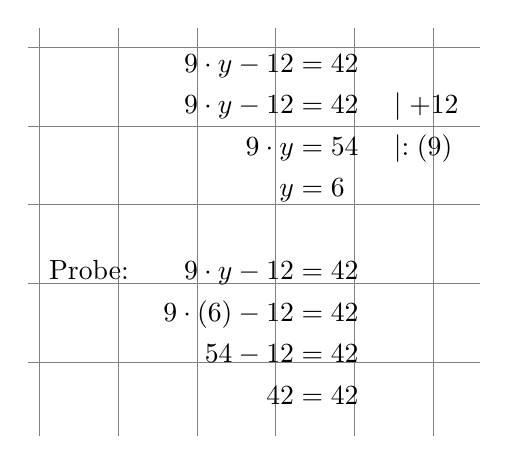
\begin{tikzpicture}[show background grid]
\node[below right] at (0,0.1) {
$\begin{aligned}
9\cdot y-12 &=42& &  \\
9\cdot y - 12 &=42& & \mid + 12\\
9\cdot y &=54& & \mid :\left(9\right)\\
y &=6& & 
\\
\\
\mbox{Probe:}\qquad 9\cdot y-12 &=42& &  \\
9\cdot \left(6\right)-12 &=42& &  \\
54-12 &=42& &  \\
42 &=42& &  \\
\end{aligned}$};
\end{tikzpicture}
\endgroup
\\\hline
u)&\begingroup\setlength{\jot}{-0.03cm}
\tikzstyle{background grid}=[draw, black!15,step=.5cm]
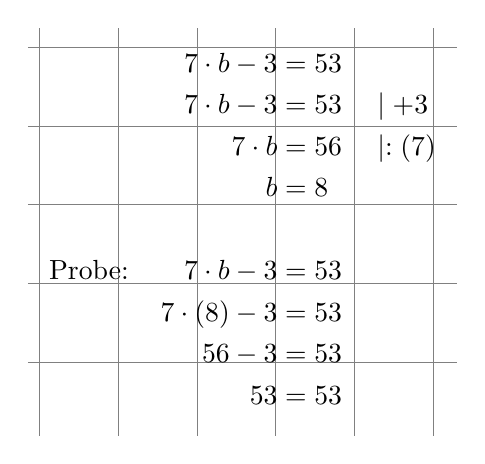
\begin{tikzpicture}[show background grid]
\node[below right] at (0,0.1) {
$\begin{aligned}
7\cdot b-3 &=53& &  \\
7\cdot b - 3 &=53& & \mid + 3\\
7\cdot b &=56& & \mid :\left(7\right)\\
b &=8& & 
\\
\\
\mbox{Probe:}\qquad 7\cdot b-3 &=53& &  \\
7\cdot \left(8\right)-3 &=53& &  \\
56-3 &=53& &  \\
53 &=53& &  \\
\end{aligned}$};
\end{tikzpicture}
\endgroup
&
v)&\begingroup\setlength{\jot}{-0.03cm}
\tikzstyle{background grid}=[draw, black!15,step=.5cm]
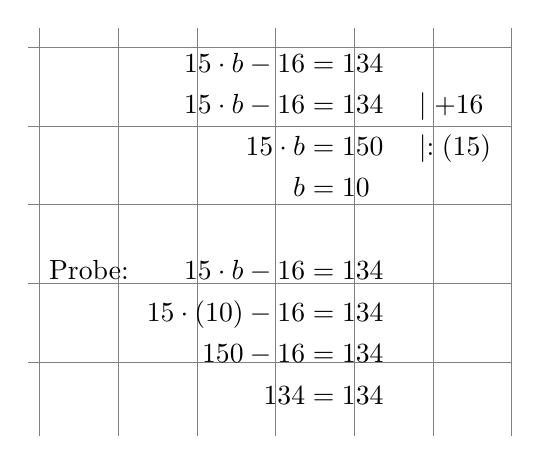
\begin{tikzpicture}[show background grid]
\node[below right] at (0,0.1) {
$\begin{aligned}
15\cdot b-16 &=134& &  \\
15\cdot b - 16 &=134& & \mid + 16\\
15\cdot b &=150& & \mid :\left(15\right)\\
b &=10& & 
\\
\\
\mbox{Probe:}\qquad 15\cdot b-16 &=134& &  \\
15\cdot \left(10\right)-16 &=134& &  \\
150-16 &=134& &  \\
134 &=134& &  \\
\end{aligned}$};
\end{tikzpicture}
\endgroup
\\\hline
w)&\begingroup\setlength{\jot}{-0.03cm}
\tikzstyle{background grid}=[draw, black!15,step=.5cm]
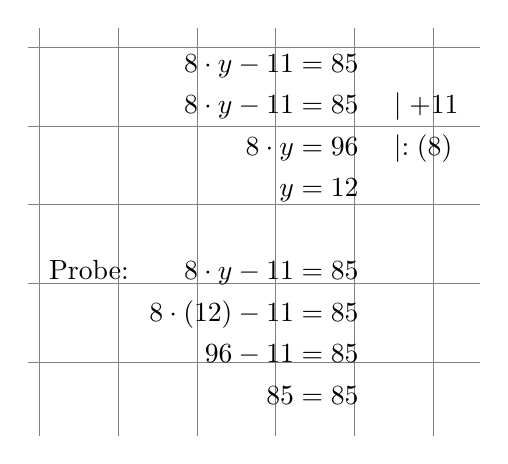
\begin{tikzpicture}[show background grid]
\node[below right] at (0,0.1) {
$\begin{aligned}
8\cdot y-11 &=85& &  \\
8\cdot y - 11 &=85& & \mid + 11\\
8\cdot y &=96& & \mid :\left(8\right)\\
y &=12& & 
\\
\\
\mbox{Probe:}\qquad 8\cdot y-11 &=85& &  \\
8\cdot \left(12\right)-11 &=85& &  \\
96-11 &=85& &  \\
85 &=85& &  \\
\end{aligned}$};
\end{tikzpicture}
\endgroup
&
x)&\begingroup\setlength{\jot}{-0.03cm}
\tikzstyle{background grid}=[draw, black!15,step=.5cm]
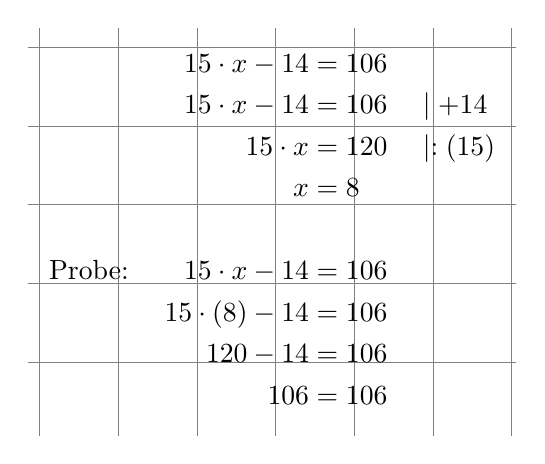
\begin{tikzpicture}[show background grid]
\node[below right] at (0,0.1) {
$\begin{aligned}
15\cdot x-14 &=106& &  \\
15\cdot x - 14 &=106& & \mid + 14\\
15\cdot x &=120& & \mid :\left(15\right)\\
x &=8& & 
\\
\\
\mbox{Probe:}\qquad 15\cdot x-14 &=106& &  \\
15\cdot \left(8\right)-14 &=106& &  \\
120-14 &=106& &  \\
106 &=106& &  \\
\end{aligned}$};
\end{tikzpicture}
\endgroup
\\\hline
y)&\begingroup\setlength{\jot}{-0.03cm}
\tikzstyle{background grid}=[draw, black!15,step=.5cm]
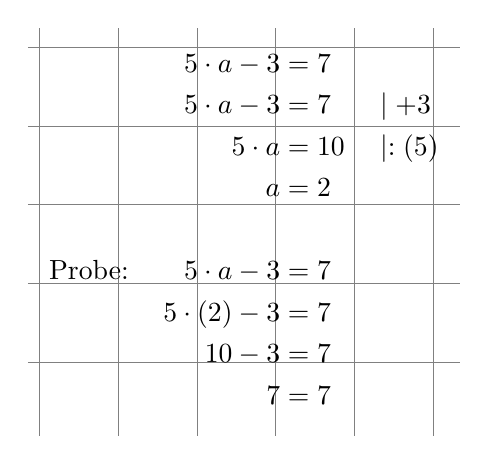
\begin{tikzpicture}[show background grid]
\node[below right] at (0,0.1) {
$\begin{aligned}
5\cdot a-3 &=7& &  \\
5\cdot a - 3 &=7& & \mid + 3\\
5\cdot a &=10& & \mid :\left(5\right)\\
a &=2& & 
\\
\\
\mbox{Probe:}\qquad 5\cdot a-3 &=7& &  \\
5\cdot \left(2\right)-3 &=7& &  \\
10-3 &=7& &  \\
7 &=7& &  \\
\end{aligned}$};
\end{tikzpicture}
\endgroup
&
z)&\begingroup\setlength{\jot}{-0.03cm}
\tikzstyle{background grid}=[draw, black!15,step=.5cm]
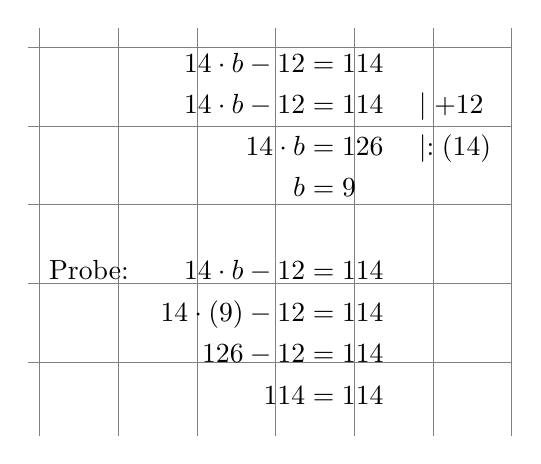
\begin{tikzpicture}[show background grid]
\node[below right] at (0,0.1) {
$\begin{aligned}
14\cdot b-12 &=114& &  \\
14\cdot b - 12 &=114& & \mid + 12\\
14\cdot b &=126& & \mid :\left(14\right)\\
b &=9& & 
\\
\\
\mbox{Probe:}\qquad 14\cdot b-12 &=114& &  \\
14\cdot \left(9\right)-12 &=114& &  \\
126-12 &=114& &  \\
114 &=114& &  \\
\end{aligned}$};
\end{tikzpicture}
\endgroup
\\\hline
\end{xltabular}
\vspace{0.5cm}
\end{document}